\section{射影簇之间的正则映射}\label{sec:regular-maps-of-projective-varieties}

本节的目标是熟悉两个射影簇之间正则映射的精确概念. 如本章引言中所提到的, 射影簇之间的正则映射局部以一组同次数的齐次多项式为模型. 在给出关键定义前, 先作几点观察.

设 $f\in K[x_{0},\ldots,x_{m}]$ 且 $a\in\mathbb{P}^{m}$. 选取齐次坐标并写成 $a=[a_{0}:\cdots:a_{m}]$ 后, 可以对 $f$ 求值得到
\[
  f(a_{0},\ldots,a_{m})\in K.
\]
然而, 正如我们已经看到的, 选取 $a$ 的不同齐次坐标会使对 $f$ 求值得到不同的值, 因此 $f$ 在 $\mathbb{P}^{m}$ 的点处的值不是良定义的. 为了绕开这一问题, 不妨假设 $f_{0},\ldots,f_{n}\in K[x_{0},\ldots,x_{m}]$ 都是 $d$ 次齐次多项式, 且至少一个不在 $a$ 消没. 这样可以把各个值放在一起, 把它们视为射影空间中的一个点:
\[
  [f_{0}(a_{0},\ldots,a_{m}):\cdots:f_{n}(a_{0},\ldots,a_{m})]\in\mathbb{P}^{n}.
\]
这样做带来了一个很好的结果: $\mathbb{P}^{n}$ 中的相应点实际上与 $a$ 的齐次坐标的选取无关. 的确, 若选取任意另一组齐次坐标 $a=[\lambda a_{0}:\cdots:\lambda a_{m}]$, 则
\[
  \begin{aligned}
  &[f_{0}(\lambda a_{0},\ldots,\lambda a_{m}):\cdots:f_{n}(\lambda a_{0},\ldots,\lambda a_{m})]\\
  &\qquad=[\lambda^{d}f_{0}(a_{0},\ldots,a_{m}):\cdots:\lambda^{d}f_{n}(a_{0},\ldots,a_{m})]\\
  &\qquad=[f_{0}(a_{0},\ldots,a_{m}):\cdots:f_{n}(a_{0},\ldots,a_{m})],
  \end{aligned}
\]
其中第一个等式利用各 $f_{i}$ 的齐次性, 第二个等式利用 $\mathbb{P}^{n}$ 中的等价关系. 在这种情形下, 此后采用简写
\[
  [f_{0}(a):\cdots:f_{n}(a)]=[f_{0}(a_{0},\ldots,a_{m}):\cdots:f_{n}(a_{0},\ldots,a_{m})],
\]
由于单个值 $f_{i}(a)$ 并非良定义, 这里略微滥用了记号. 在 $\mathbb{P}^{m}$ 中所有至少一个 $f_{i}$ 不消没的点处求值, 便得到函数
\[
  [f_{0}:\cdots:f_{n}]:\mathbb{P}^{m}\setminus\mathcal{V}(f_{0},\ldots,f_{n})\to\mathbb{P}^{n}.
\]
这样得到的函数自然引出射影簇之间的多项式映射概念. 这是我们在本节稍后引入的更一般的正则映射概念的初步形式.

\begin{Definition}{射影簇之间的多项式映射}\leavevmode\label{def:polynomial-maps-between-projective-varieties}
设 $X\subseteq\mathbb{P}^{m}$ 和 $Y\subseteq\mathbb{P}^{n}$ 为射影簇. 如果存在同次数的齐次多项式 $f_{0},\ldots,f_{n}\in K[x_{0},\ldots,x_{m}]$, 使得 $X\cap\mathcal{V}(f_{0},\ldots,f_{n})=\varnothing$ 且
\[
  F(a)=[f_{0}(a):\cdots:f_{n}(a)]\qquad\text{对所有 }a\in X,
\]
就称映射 $F:X\to Y$ 为\emph{多项式映射}. 若 $f_{0},\ldots,f_{n}$ 可以取为线性的, 就称 $F$ 为\emph{线性映射}.
\end{Definition}

所要求的两个条件, 即 $f_{0},\ldots,f_{n}$ 同次数且齐次, 以及 $X\cap\mathcal{V}(f_{0},\ldots,f_{n})=\varnothing$, 一起保证对每个 $a\in X$, $[f_{0}(a):\cdots:f_{n}(a)]$ 是 $\mathbb{P}^{n}$ 中良定义的点. 下面看几个具体例子.

\begin{Example}{从 $\mathbb{P}^{1}$ 到一条二次曲线的多项式映射}\leavevmode\label{ex:polynomial-map-from-projective-line-to-conic}
令 $X=\mathcal{V}(y^{2}-xz)\subseteq\mathbb{P}^{2}$, 考察函数
\[
  \begin{aligned}
    G:\mathbb{P}^{1}&\to X\\
    [a:b]&\mapsto[a^{2}:ab:b^{2}].
  \end{aligned}
\]
这是一个多项式映射: 用定义域的坐标 $s,t$ 表示, $G=[s^{2}:st:t^{2}]$. 由
\[
  \mathcal{V}(s^{2},st,t^{2})=\varnothing\subseteq\mathbb{P}^{1}
\]
可知 $G$ 在 $\mathbb{P}^{1}$ 的每一点都有定义. 为了验证 $G$ 的像落在 $X$ 内, 注意对任意 $[a:b]\in\mathbb{P}^{1}$, $X$ 的定义方程 $y^{2}-xz$ 在 $[a^{2}:ab:b^{2}]$ 处取值为零.
\end{Example}

\begin{Example}{从二次曲面到 $\mathbb{P}^{2}$ 的线性映射}\leavevmode\label{ex:linear-map-from-projective-quadric}
令 $X=\mathcal{V}(w^{2}+x^{2}+y^{2}-z^{2})\subseteq\mathbb{P}^{3}$. 由于 $[0:0:0:1]\notin X$, 得到线性映射
\[
  \begin{aligned}
    H:X&\to\mathbb{P}^{2}\\
    [a:b:c:d]&\mapsto[a:b:c],
  \end{aligned}
\]
它由齐次线性多项式 $w,x,y\in K[w,x,y,z]$ 给出.

\BookPairedFigure{
为了直观理解 $H$, 考察 $X$ 在 $w\ne0$ 的仿射开片 $\mathbb{A}^{3}_{0}$ 上的限制:
\[
  X_{0}=\mathcal{V}(1+x^{2}+y^{2}-z^{2})\subseteq\mathbb{A}^{3}.
\]
限制在这个开片时, 映射 $H$ 把 $(b,c,d)\in X_{0}$ 送到 $(b,c)\in\mathbb{A}^{2}$. 在实数域上, 可以直观地把它看成把右图中的双叶双曲面竖直投影到水平坐标平面上的二对一映射.
}{
\phantomsection\label{fig:projective-quadric-linear-projection}%
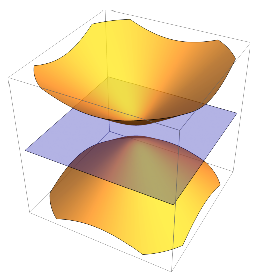
\includegraphics[width=\linewidth]{figures/projective-quadric-linear-projection.pdf}
}
\end{Example}

\begin{Example}{线性投影}\leavevmode\label{ex:linear-projections-of-projective-varieties}
推广前一例, 设 $X\subseteq\mathbb{P}^{n}$ 是不包含点 $[0:\cdots:0:1]$ 的射影簇. $X$ 到 $\mathbb{P}^{n-1}$ 的\emph{线性投影}是线性映射
\[
  \begin{aligned}
    H:X&\to\mathbb{P}^{n-1}\\
    [a_{0}:\cdots:a_{n-1}:a_{n}]&\mapsto[a_{0}:\cdots:a_{n-1}].
  \end{aligned}
\]
可以这样直观理解 $H$: 给定点 $a=[a_{0}:\cdots:a_{n}]\in X$, 存在唯一一条经过 $[0:\cdots:0:1]$ 和 $a$ 的直线 $L_{a}\subseteq\mathbb{P}^{n}$:
\[
  L_{a}=\{[ca_{0}:\cdots:ca_{n-1}:da_{n}]\mid[c:d]\in\mathbb{P}^{1}\}.
\]
这条直线与超平面 $\mathcal{V}(x_{n})\subseteq\mathbb{P}^{n}$ 相交于点 $[a_{0}:\cdots:a_{n-1}:0]$. 将 $\mathcal{V}(x_{n})$ 与 $\mathbb{P}^{n-1}$ 自然等同, 这个交点就是 $H(a)$. 因此, 可以直观地把 $H(X)$ 看作从 $[0:\cdots 0:1]$ 照来的光在 $\mathcal{V}(x_{n})$ 上投下的 $X$ 的影子. 在 $x_{0}\ne0$ 的仿射开片上, 直线 $L_{a}$ 是仅有最后一个坐标变化的\textquotedbl{}竖直\textquotedbl{}直线, 超平面 $\mathcal{V}(x_{n})$ 则是最后一个坐标为零的\textquotedbl{}水平\textquotedbl{}超平面. 因此, 如 Example~\ref{ex:linear-map-from-projective-quadric} 所示, 在这一开片内线性投影就是竖直投影.
\end{Example}

为了引出更一般的正则映射的定义, 注意 Definition~\ref{def:polynomial-maps-between-projective-varieties} 中 $X\cap\mathcal{V}(f_{0},\ldots,f_{n})=\varnothing$ 的限制常常过强. 允许映射只在\textquotedbl{}局部\textquotedbl{}用多项式描述, 会为我们提供有用的灵活性. 为了更好地理解这一点, 来看一个例子.

\begin{Example}{从二次曲线到 $\mathbb{P}^{1}$ 的分片多项式函数}\leavevmode\label{ex:piecewise-polynomial-map-from-conic}
令 $X=\mathcal{V}(y^{2}-xz)\subseteq\mathbb{P}^{2}$, 考察一对齐次线性多项式 $x,y\in K[x,y,z]$. 注意这些多项式并不给出从 $X$ 到 $\mathbb{P}^{1}$ 的多项式映射, 原因仅仅是 $\mathcal{V}(x,y)\cap X=\{[0:0:1]\}\ne\varnothing$. 不过, 我们仍得到从 $X$ 的一个子集到 $\mathbb{P}^{1}$ 的函数:
\[
  \begin{aligned}
    [x:y]:X\setminus\mathcal{V}(x,y)&\to\mathbb{P}^{1}\\
    [a:b:c]&\mapsto[a:b].
  \end{aligned}
\]
重要的是, 我们关心的不是多项式对 $(x,y)$, 而是这对多项式定义的函数 $[x:y]$. 例如, 函数 $[5x:5y]$ 与 $[x:y]$ 相同, 只因为缩放坐标不会改变 $\mathbb{P}^{1}$ 中的点. 更一般地, 回顾 $\mathbb{P}^{1}$ 中两点 $[a:b]$ 和 $[a':b']$ 相等当且仅当它们的交叉乘积 $ab'$ 和 $ba'$ 相等 (Exercise~\ref{ex:cross-multiplied-projective-coordinates}). 于是, $X$ 上的两个函数 $[f:g]$ 和 $[f':g']$ 在它们都有定义的每一点相等, 当且仅当它们的交叉乘积在 $X$ 上相等:
\[
  fg'-gf'\in\mathcal{I}(X).
\]
例如, 映射 $[x:y]$ 和 $[y:z]$ 在 $X$ 内共同定义域的每一点相等, 因为它们的交叉乘积之差是 $xz-y^{2}$, 它在 $X$ 上消没. 那么, 考察第二个函数:
\[
  \begin{aligned}
    [y:z]:X\setminus\mathcal{V}(y,z)&\to\mathbb{P}^{1}\\
    [a:b:c]&\mapsto[b:c].
  \end{aligned}
\]
注意 $[x:y]$ 和 $[y:z]$ 的定义域合起来覆盖整个 $X$, 因为第一个定义域只漏掉 $[0:0:1]$, 而第二个只漏掉 $[1:0:0]$. 由于这两个映射在它们都有定义的每一点相等, 就可以把它们合起来, 得到整个 $X$ 上分片定义的函数:
\[
  \begin{aligned}
    F:X&\to\mathbb{P}^{1}\\
    [a:b:c]&\mapsto
    \begin{cases}
      [a:b] & \text{若 }[a:b:c]\notin\mathcal{V}(x,y),\\
      [b:c] & \text{若 }[a:b:c]\notin\mathcal{V}(y,z).
    \end{cases}
  \end{aligned}
\]
\end{Example}

前例中的函数 $F:X\to\mathbb{P}^{1}$ 不能由单独一对多项式描述, 但它在以下意义上是\textquotedbl{}局部\textquotedbl{}多项式的: 对每个点 $p\in X$, 都存在一对 $f,g\in K[x,y,z]$, 不同的点可能对应不同的多项式对, 使得 $p\notin\mathcal{V}(f,g)$ 且
\[
  F(a)=[f(a):g(a)]\qquad\text{对所有 }a\in X\setminus\mathcal{V}(f,g).
\]
$F$ 的这一刻画引出了正则映射的定义.

\begin{Definition}{射影簇之间的正则映射}\leavevmode\label{def:regular-maps-between-projective-varieties}
设 $X\subseteq\mathbb{P}^{m}$ 和 $Y\subseteq\mathbb{P}^{n}$ 为射影簇. 如果对每个 $p\in X$, 均存在同次数的齐次多项式 $f_{0},\ldots,f_{n}\in K[x_{0},\ldots,x_{m}]$, 使得 $p\notin\mathcal{V}(f_{0},\ldots,f_{n})$ 且
\[
  F(a)=[f_{0}(a):\cdots:f_{n}(a)]
  \qquad\text{对所有 }a\in X\setminus\mathcal{V}(f_{0},\ldots,f_{n}),
\]
就称映射 $F:X\to Y$ 为\emph{正则映射}.
\end{Definition}

换句话说, 若对每个 $p\in X$ 都可以为 $F$ 找到一个在 $p$ 处良定义的多项式表达式, 即使这个表达式可能不在整个 $X$ 上良定义, $F:X\to Y$ 也是正则的. 由定义可知, 每个多项式映射都是正则的, 但反过来不成立: 并非每个正则映射都能在整体上用单独一组多项式描述. 下一个例子验证这一事实.

\begin{Example}{不是多项式映射的正则映射}\leavevmode\label{ex:regular-map-not-polynomial-map}
令 $X=\mathcal{V}(y^{2}-xz)\subseteq\mathbb{P}^{2}$, 再次考察 Example~\ref{ex:piecewise-polynomial-map-from-conic} 的正则映射:
\[
  \begin{aligned}
    F:X&\to\mathbb{P}^{1}\\
    [a:b:c]&\mapsto
    \begin{cases}
      [a:b] & [a:b:c]\notin\mathcal{V}(x,y),\\
      [b:c] & [a:b:c]\notin\mathcal{V}(y,z).
    \end{cases}
  \end{aligned}
\]
我们断言 $F$ 不是多项式映射. 为了说明这一点, 反设存在同为 $d$ 次的齐次多项式 $f,g\in K[x,y,z]$, 使 $\mathcal{V}(f,g)\cap X=\varnothing$ 且 $F=[f:g]$. 用 Example~\ref{ex:polynomial-map-from-projective-line-to-conic} 中的映射 $G$ 与 $F$ 复合 (先作用 $G$), 得到映射 $F\circ G:\mathbb{P}^{1}\to\mathbb{P}^{1}$. 一方面, 容易验证 $F\circ G$ 是 $\mathbb{P}^{1}$ 上的恒等映射 (见下一节的 Example~\ref{ex:projective-line-isomorphic-to-conic}); 另一方面, $F\circ G$ 也可以用 $f$ 和 $g$ 显式写成
\[
  (F\circ G)([a:b])=F([a^{2}:ab:b^{2}])=[f(a^{2},ab,b^{2}):g(a^{2},ab,b^{2})].
\]
因此, 若定义 $f_{0}(s,t)=f(s^{2},st,t^{2})$ 及 $g_{0}(s,t)=g(s^{2},st,t^{2})$, 则 $f_{0}$ 和 $g_{0}$ 都是 $K[s,t]$ 中 $2d$ 次的齐次多项式, 并定义了与恒等映射相同的多项式映射 $[f_{0}:g_{0}]:\mathbb{P}^{1}\to\mathbb{P}^{1}$. 然而, 这就产生了矛盾, 因为任何定义了 $\mathbb{P}^{1}$ 上恒等映射的多项式映射都必须具有 $f_{0}=as$ 和 $g_{0}=at$ 的形式, 其中 $a\in K$ 非零 (Exercise~\ref{ex:polynomial-representatives-of-projective-identity}). 特别地, $f_{0}$ 和 $g_{0}$ 必须是线性的, 故它们不可能对任何 $d$ 有次数 $2d$. 这一矛盾意味着 $F$ 不是多项式映射, 如所断言.
\end{Example}

最后指出, 描述正则映射的一般方法是分片定义它, 正如在 Example~\ref{ex:piecewise-polynomial-map-from-conic} 中所做的那样. 更准确地说, 射影簇 $X\subseteq\mathbb{P}^{m}$ 和 $Y\subseteq\mathbb{P}^{n}$ 之间的正则映射 $F:X\to Y$, 按定义总能用一族如下形式的函数描述:
\[
  [f_{0}:\cdots:f_{n}]:X\setminus\mathcal{V}(f_{0},\ldots,f_{n})\to Y.
\]
这族函数必须满足以下两个性质:
\begin{enumerate}[label=\arabic*.]
  \item 若 $[f_{0}:\cdots:f_{n}]$ 和 $[g_{0}:\cdots:g_{n}]$ 都在该族中, 则
  \[
    f_{i}g_{j}-f_{j}g_{i}\in\mathcal{I}(X)\qquad\text{对所有 }i,j.
  \]
  \item 每个 $p\in X$ 都必须属于该族中至少一个函数的定义域.
\end{enumerate}
第一项条件保证该族中的两个函数在共同定义域上相等, 因而可以合并它们, 得到定义域的并上的良定义函数. 第二项条件保证所有定义域的并覆盖 $X$. 事实上, 虽然从定义并不能直接看出这一点, 读者不妨验证: 每个正则映射不仅能用一族这样的函数描述, 而且能用\emph{有限}族这样的函数描述 (Exercise~\ref{ex:finite-polynomial-representations-cover-regular-map}).

\BookExerciseHeading
\begin{BookExercises}
  \item\label{ex:restrict-regular-map-to-projective-subvariety} 设 $X\subseteq\mathbb{P}^{m}$ 和 $Y\subseteq\mathbb{P}^{n}$ 为射影簇, $F:X\to Y$ 为正则映射. 若 $Z\subseteq\mathbb{P}^{m}$ 是满足 $Z\subseteq X$ 的任一射影簇, 解释为什么限制映射 $F|_{Z}:Z\to Y$ 也是正则映射.
  \item\label{ex:composition-of-projective-regular-maps} 设 $X\subseteq\mathbb{P}^{\ell}$, $Y\subseteq\mathbb{P}^{m}$, $Z\subseteq\mathbb{P}^{n}$ 均为射影簇. 若 $F:X\to Y$ 和 $G:Y\to Z$ 是正则映射, 证明 $G\circ F:X\to Z$ 也是正则的.
  \item\label{ex:regular-projection-from-projective-quadric} 令 $X=\mathcal{V}(wz-xy)\subseteq\mathbb{P}^{3}$.
  \begin{enumerate}
    \item 构造延拓函数
    \[
      [w:x]:X\setminus\mathcal{V}(w,x)\to\mathbb{P}^{1}
    \]
    的正则映射 $F:X\to\mathbb{P}^{1}$.
    \item 证明 $F$ 是满射.
    \item 对任意 $b\in\mathbb{P}^{1}$, 计算原像
    \[
      F^{-1}(b)=\{a\in X\mid F(a)=b\}.
    \]
  \end{enumerate}
  \item\label{ex:regular-map-from-projective-line-is-polynomial} 证明每个正则映射 $F:\mathbb{P}^{1}\to\mathbb{P}^{n}$ 都是多项式映射.
  \item\label{ex:coordinate-projection-does-not-extend-to-center} 证明映射
  \[
    [x_{0}:\cdots:x_{n-1}]:\mathbb{P}^{n}\setminus\mathcal{V}(x_{0},\ldots,x_{n-1})\to\mathbb{P}^{n-1}
  \]
  不能延拓为整个 $\mathbb{P}^{n}$ 上的正则映射.
  \item\label{ex:polynomial-representatives-of-projective-identity} 令 $f,g\in K[x,y]$ 为同次数的齐次多项式, 且 $\mathcal{V}(f,g)=\varnothing$, 并假设多项式映射 $[f:g]:\mathbb{P}^{1}\to\mathbb{P}^{1}$ 是恒等映射. 证明存在非零 $a\in K$, 使 $f=ax$ 且 $g=ay$.
  \item\label{ex:projective-linear-projection-is-finite-to-one} 设 $X\subseteq\mathbb{P}^{n}$ 为不包含 $[0:\cdots:0:1]$ 的射影簇, 考察线性投影
  \[
    \begin{aligned}
      H:X&\to\mathbb{P}^{n-1}\\
      [a_{0}:\cdots:a_{n-1}:a_{n}]&\mapsto[a_{0}:\cdots:a_{n-1}].
    \end{aligned}
  \]
  证明 $H$ 是有限对一的. 换句话说, 证明对任意 $b\in\mathbb{P}^{n-1}$, 原像 $H^{-1}(b)=\{a\in X\mid H(a)=b\}$ 是有限集.
  \item\label{ex:finite-polynomial-representations-cover-regular-map} 设 $X\subseteq\mathbb{P}^{m}$ 和 $Y\subseteq\mathbb{P}^{n}$ 为射影簇, $F:X\to Y$ 为正则映射. 证明存在一有限族如下形式的函数:
  \[
    [f_{0}:\cdots:f_{n}]:X\setminus\mathcal{V}(f_{0},\ldots,f_{n})\to Y,
  \]
  使得
  \begin{itemize}
    \item 该族中每个函数在自身定义域上都与 $F$ 相同, 并且
    \item $X$ 的每一点都属于该族中至少一个函数的定义域.
  \end{itemize}
\end{BookExercises}

\par\medskip
{\footnotesize
\noindent\textbf{开放获取.} 本章按照
\href{http://creativecommons.org/licenses/by-nc/4.0/}{Creative Commons Attribution-NonCommercial 4.0 International License}
的条款授权. 该许可允许以任何媒介或格式进行非商业性使用, 分享, 改编, 分发和复制, 但须对原作者和来源作适当署名, 提供 Creative Commons 许可的链接, 并说明是否作了修改.

\noindent
\begin{minipage}[t]{.17\linewidth}
  \vspace{0pt}
\includegraphics[width=.9\linewidth]{figures/source-cc-by-nc.png}
\end{minipage}\hfill
\begin{minipage}[t]{.81\linewidth}
  \vspace{0pt}本章的图片或其他第三方材料均纳入本章的 Creative Commons 许可, 除非材料的署名行另有注明. 如果材料未纳入本章的 Creative Commons 许可, 且您拟进行的使用未获法律规定的许可或超出允许使用的范围, 则须直接向著作权持有人取得许可.
\end{minipage}\par}
